\documentclass[13pt]{extarticle}

\usepackage[T1]{fontenc}
\usepackage[utf8]{inputenc}
\usepackage[russian]{babel}

% page margin
\usepackage[top=2cm, bottom=2cm, left=2cm, right=2cm]{geometry}

% AMS packages
\usepackage{amsmath}
\usepackage{amssymb}
\usepackage{amsfonts}
\usepackage{amsthm}

\usepackage{float}
\usepackage{graphicx}
\usepackage{tabularx}
\usepackage{multirow}

\newcommand{\lb}{\left(}
\newcommand{\rb}{\right)}

\makeatletter
\setlength{\@fptop}{0pt}
\makeatother

\DeclareMathOperator{\arcsinh}{arcsinh}

\begin{document}

\subsection*{Расчет емкости плотного слоя воды на поверхности электрода Au$(111)$ в рамках модели Грэма}

В растворе поверхностно-неактивного электролита в гальвани-потенциале $\Delta \phi$ выделяют следующие три составляющие:
\begin{enumerate}
	\item разность потенциалов, обусловленная выходом электронной плотности за пределы ионного остава металла
	\item разность потенциалов, вызванная некоторой предпочтительной ориентацией примыкающих к электроду диполей растворителя
	\item разность потенциалов (ионный скачок потенциала), обусловленная зарядом электрода $q$ и компенсирующими этот заряд ионами раствора. Выделяют $\Delta \varphi_H$ (от поверхности металла $x = 0$ до внешней плоскости Гельмгольца $x = x_2$) и $\Delta \varphi_2$ (падение потенциала в диффузном слое).
\end{enumerate}

Согласно модели Грэма суммарное значение разности потенциалов разбивается следующим образом:
\begin{gather}
	\varphi_0 = \varphi_{02} + \varphi_{2} \notag \\
	\frac{1}{C} = \frac{1}{C_{02}} + \frac{1}{C_2} \label{grem} 
\end{gather}

Это разбиение обусловлено тем, что при $T = $const величины $\varphi_{02}, C_{02}$ не зависят от концентрации раствора, а величины $\varphi_2, C_2$ не зависят от природы металла. Потенциал $\varphi_2$ оказывается связанным с зарядом электрода $q$ соотношением \eqref{phi_to_q}, а соответствующая емкость $C_2$ с зарядом электрода $q$ -- посредством \eqref{c2_to_q}.
\begin{gather}
	\varphi_2 = \frac{2RT}{F} \arcsinh \frac{q}{2 A \sqrt{c}} \label{phi_to_q} \\
	C_2 = \frac{F}{2 R T} \sqrt{4 A^2 c + q^2} \label{c2_to_q}, \quad A = \sqrt{2 R T \varepsilon_0 \varepsilon}
\end{gather}

Данные по зависимости емкости $C$ от потенциала $\varphi$ были взяты из статьи [1] (рис. 8а, линия 1). В результате оцифровки рисунка был получен массив точек, который был профитован кубическим сплайном (Рис. \ref{kolb1986}).
\begin{figure}[!ht]
	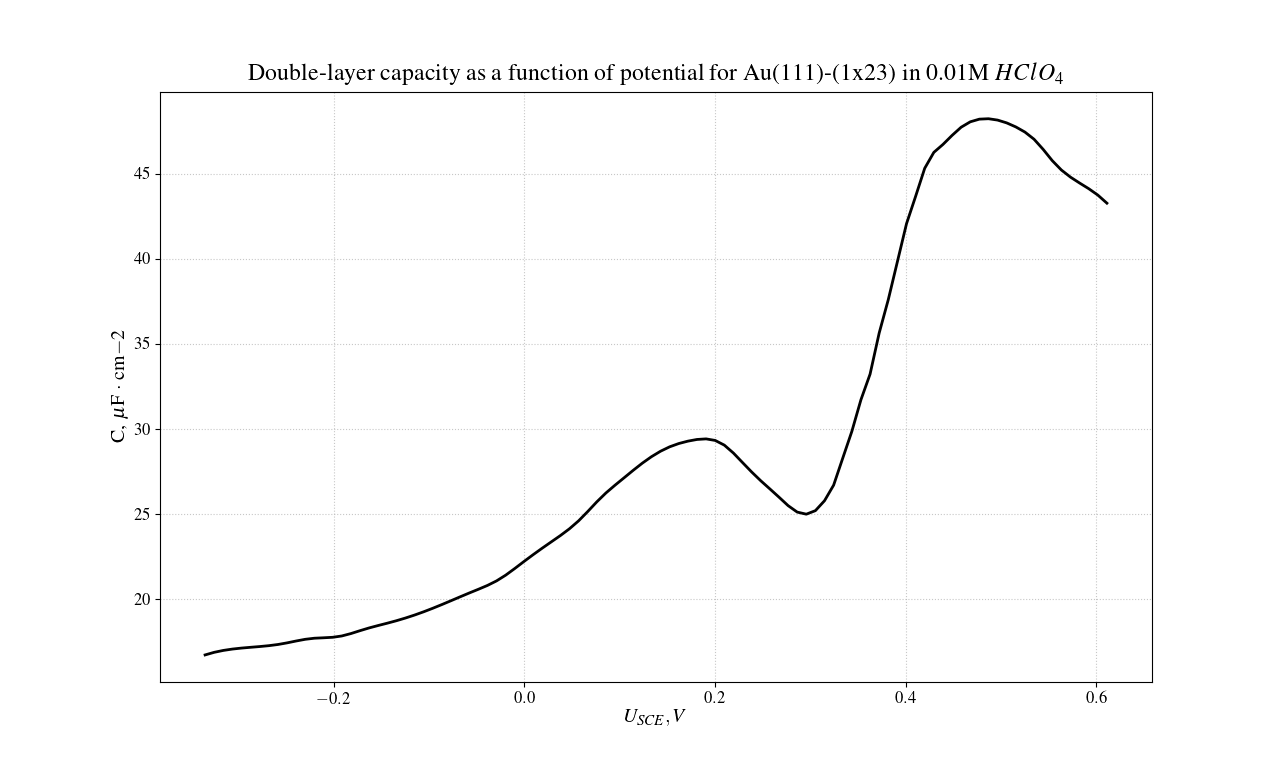
\includegraphics[width = \linewidth]{../pictures/kolb1986_8figure.png}
	\caption{Оцифрованные данные из статьи [1]}
	\label{kolb1986}
\end{figure}

В тексте [1] приведено значение потенциала нулевого заряда \textit{pzc} = $+ 0.32$ В. Зависимость заряда электрода $q$ от потенциала $\varphi$ (Рис. \ref{q_phi} -- красным отмечена \textit{pzc}) была рассчитана по следующей формуле
\begin{gather}
	q(\varphi) = \int\limits_{\textit{pzc}}^{\varphi} C \lb \varphi^\prime \rb d \varphi^\prime \notag
\end{gather}

\begin{figure}[!ht]
	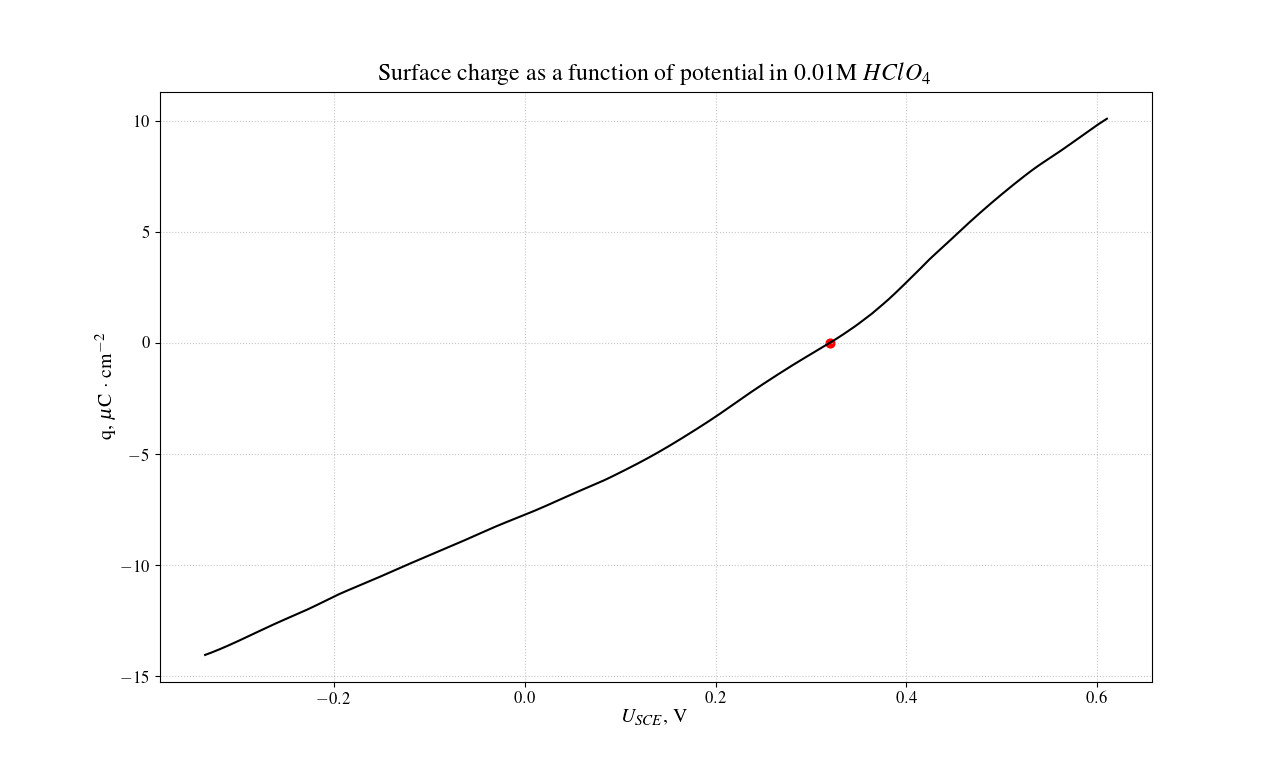
\includegraphics[width = \linewidth]{../pictures/surface_charge.png}
	\caption{Зависимость поверхностого заряда $q$ от потенциала $U$}
	\label{q_phi}
\end{figure}

По соотношению \eqref{c2_to_q} получена зависимость $C_2$ от $q$, которая затем была использована для расчета зависимости $C_{02}$ от $q$ и $C_{02}$ от $\varphi$ по соотношению \eqref{grem} (Рис. \ref{dense}).

\begin{figure}[!ht]
	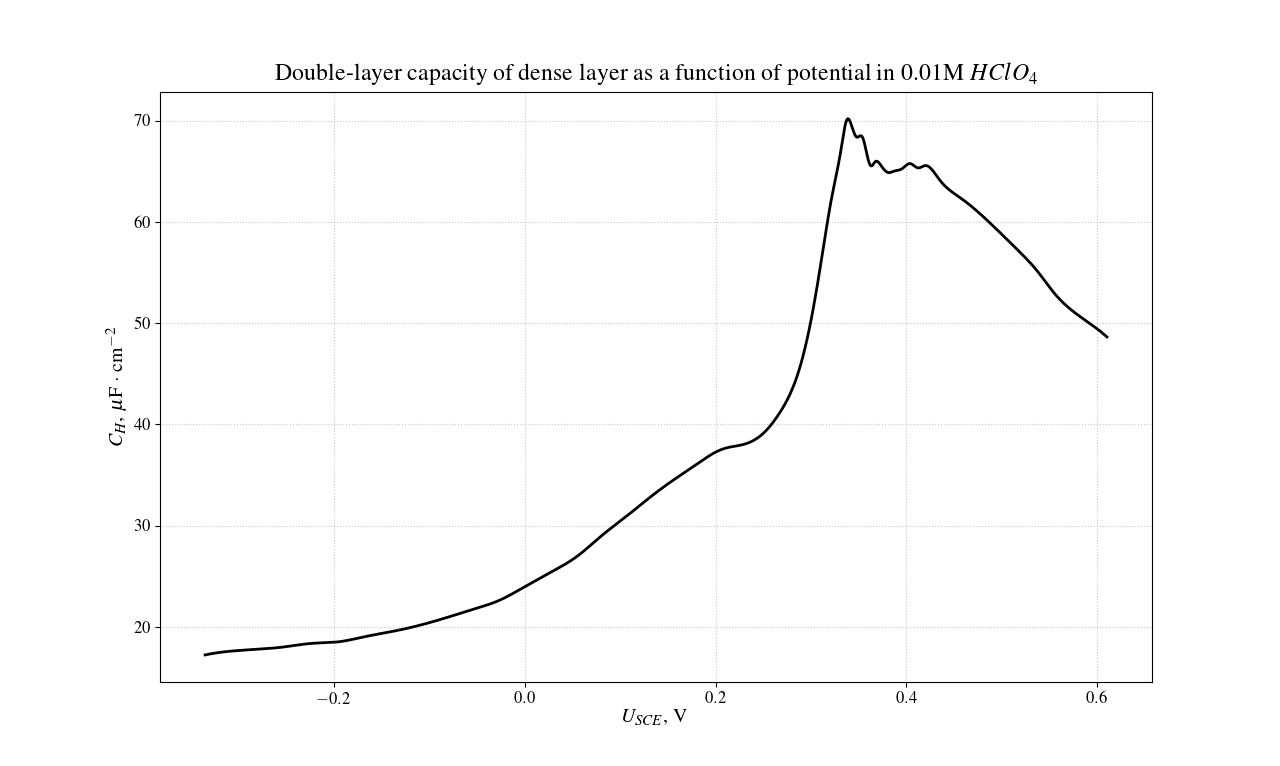
\includegraphics[width = \linewidth]{../pictures/dense_layer.png}
	\caption{Зависимость емкости плотного слоя $C_{02}$ от потенциала электрода $\varphi$} 
	\label{dense}
\end{figure}

Авторы [2] определяли параметры ультрабыстрой релаксации возбужденных электронов на поверхности электрода Au(111) в растворе $HClO_4$ (Рис. \ref{decay_rate}). В области $0.3-0.4$ В наблюдается изменение тренда в зависимости времени затухания отклика от потенциала электрода, которое авторы объясняют изменением ориентаций молекул воды в плотном приповерхностном слое, совместно с которыми изменяются направление дипольных моментов.  
\begin{figure}[!ht]
	\centering
	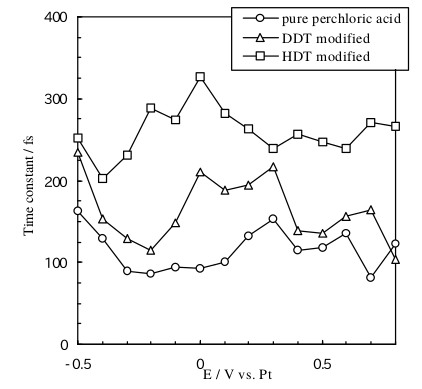
\includegraphics[width = 0.5\linewidth]{../pictures/decay_rate.png}
	\caption{Зависимость времени затухания отклика в зависимости от потенциала электрода $\varphi$}
	\label{decay_rate}
\end{figure}

\subsection*{Список литературы}

\begin{enumerate}
	\item D. M. Kolb, J. Schneider. \textit{Electrochimica Acta}, \textbf{31}, 8, 1986, 929-936 
	\item T. Sugiyama, T. Ishioka, A. Harata. \textit{Analytical Sciences}, \textbf{17}, 2001, 237-240.
\end{enumerate}

\end{document}
